\section{Background}

Big Data \& Analytics (BDA), Blockchain, and Artifical Intelligence (AI) are currently major topics in relationship to supply chain management (SCM). Google Trends shows that while interest in SCM from business and industry world-wide has remained relatively flat (see Figure \ref{fig:img1}) there has been substantial increases in interest in BDA and Blockchain, which moderate growth in interest for AI (see Figure \ref{fig:img2}). Similarly, a brief search of the Roadrunner Search Discovery Service on the topic of ``Supply Chain Management'' filtering on the terms for BDA, AI, and Blockchain yielded 3,213 peer-reviewed articles published in business journals over the year 2020 alone. A similar search for 2016 yielded only a few hundred such articles.

Off those 2020 studies, only address cost effectiveness or financial risk. Yet, there is significant disagreement as to the value these technologies can provide to organizations. For the purposes of this discussion, ``Big Data'' will be considered data that suffices the conditions of volume, variety, and velocity \parencite{hofmannBigDataSupply2017}.

\begin{figure}[h]
  \centering
  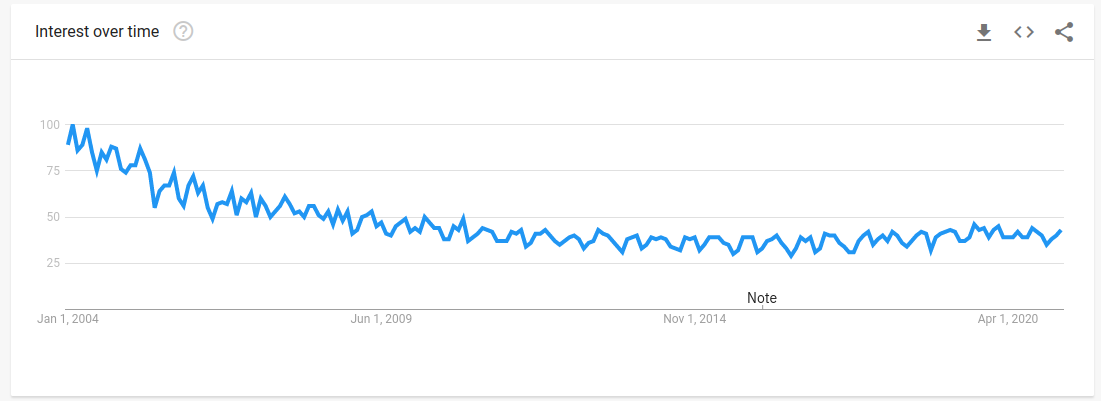
\includegraphics[width=.8\textwidth]{google1}
  \caption{Google Trend interest in Supply Chain Management}
  \label{fig:img1}
\end{figure}

\begin{figure}[h]
  \centering
  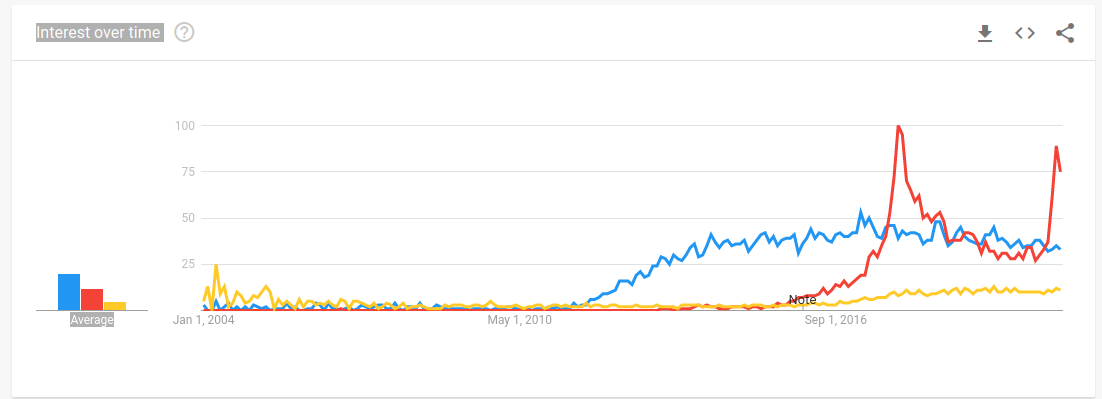
\includegraphics[width=.8\textwidth]{google2}
  \caption{Google Trend interest in BDA, AI, \& Blockchain}
  \label{fig:img2}
\end{figure}

Volume is the measure of the size of the data. It should be noted that the amount of data being discussed with respect to BDA, Blockchain, and AI involves tens or hundreds of GB of data. These volumes are not present in many BDA environments, but they are present in SCM \parencite{appuswamyNobodyEverGot2013}. In 2010, supply chains were dealing with 100GB of data daily \parencite{theeconomistDataDeluge2010}. That number is increasing annually with the proliferation of RFID and Internet of Things (IOT) \parencite{valuatesreportsRFIDMarketSize2020}. Variety is the complex nature of disparate data types including text data, image data, audio data, and so forth. Finally, velocity is the speed at which data is generated and the rate at which it must be processed to provide near-real-time information to the organization \parencite{hofmannBigDataSupply2017}.

\textcite{rossmannFutureSocialImpact2018} demonstrate that business leaders and SCM experts see little value in BDA, while computer science experts feel strongly that there is value to be had. This disagreement derives from the fact that supply chains are inherently complex, uncertain, and require significant investment in data management systems \parencite{govindanSupplyChainNetwork2017}. There is little doubt that BDA, Blockchain, and AI have the potential to enhance operational decision-making \parencite{gunasekaranInformationTechnologyCompetitive2017}. There is, however, uncertainty that he required investments necessary to drive such improvements can be recouped sufficiently \parencite{arunachalamUnderstandingBigData2018}. Similar disagreements exist for blockchain \parencite{kouhizadehBlockchainTechnologySustainable2021} and AI \parencite{nedsiArtificialIntelligenceSupply2019}
